% 
% Annual CCN conference
% Sample LaTeX Two-Page Summary -- Proceedings Format
% based on the prior cognitive science style file

% Original : Ashwin Ram (ashwin@cc.gatech.edu)       04/01/1994
% Modified : Johanna Moore (jmoore@cs.pitt.edu)      03/17/1995
% Modified : David Noelle (noelle@ucsd.edu)          03/15/1996
% Modified : Pat Langley (langley@cs.stanford.edu)   01/26/1997
% Latex2e corrections by Ramin Charles Nakisa        01/28/1997 
% Modified : Tina Eliassi-Rad (eliassi@cs.wisc.edu)  01/31/1998
% Modified : Trisha Yannuzzi (trisha@ircs.upenn.edu) 12/28/1999 (in process)
% Modified : Mary Ellen Foster (M.E.Foster@ed.ac.uk) 12/11/2000
% Modified : Ken Forbus                              01/23/2004
% Modified : Eli M. Silk (esilk@pitt.edu)            05/24/2005
% Modified : Niels Taatgen (taatgen@cmu.edu)        10/24/2006
% Modified : David Noelle (dnoelle@ucmerced.edu)     11/19/2014
% Modified : Konrad Kording (koerding@gmail.com) 2/15/2017

%% Change "letterpaper" in the following line to "a4paper" if you must. 
% Alternatively, just ignore that because who prints papers anymore?

\documentclass[10pt,letterpaper]{article}

\usepackage{ccn}
\usepackage{pslatex}
\usepackage{apacite}
\usepackage{graphicx}


\title{Neural Correlates of Context Function in Associative Learning}
 
\author{{\large \bf Samuel Gershman (gershman@fas.harvard.edu), Momchil Tomov, Hayley Dorfman}  \\
  Department of Psychology and Center for Brain Science,\\
  Harvard University, 52 Oxford St., room 295.05\\
Cambridge, MA 02138, USA}


\begin{document}

\maketitle


\begin{quote}
\small
\textbf{Keywords:} 
Bayesian modeling; Associative learning; fMRI; Neuroimaging; Context-dependent learning
\end{quote}

\section{Introduction}

The role of context during learning has been studied extensively and several conflicting views have emerged. Some studies report that the context is largely irrelevant (irrelevant context). Another view is that contexts modulate the cue-outcome associations, thus acting as occasion setters (modulatory context). Yet other studies find that the context simply acts like another punctate cue (additive context). \citeA{Gershman2017} reconciled these views in a causal structure learning model. The model captured the behavioral pattern of subjects who learned cue-outcome contingencies that were consistent with a particular context role (irrelevant, modulatory, or additive). In this study, we sought to investigate the neural correlates of context structure learning in human subjects using fMRI.

\section{Materials and Methods}

\subsubsection{Subjects.}

We recruited 28 healthy subjects (X female; Y-Z years of age; mean age Z +- SEM) to participate in this study. Eight participants were excluded due to excessive motion or insufficient data.

\begin{figure}[ht]
\begin{center}
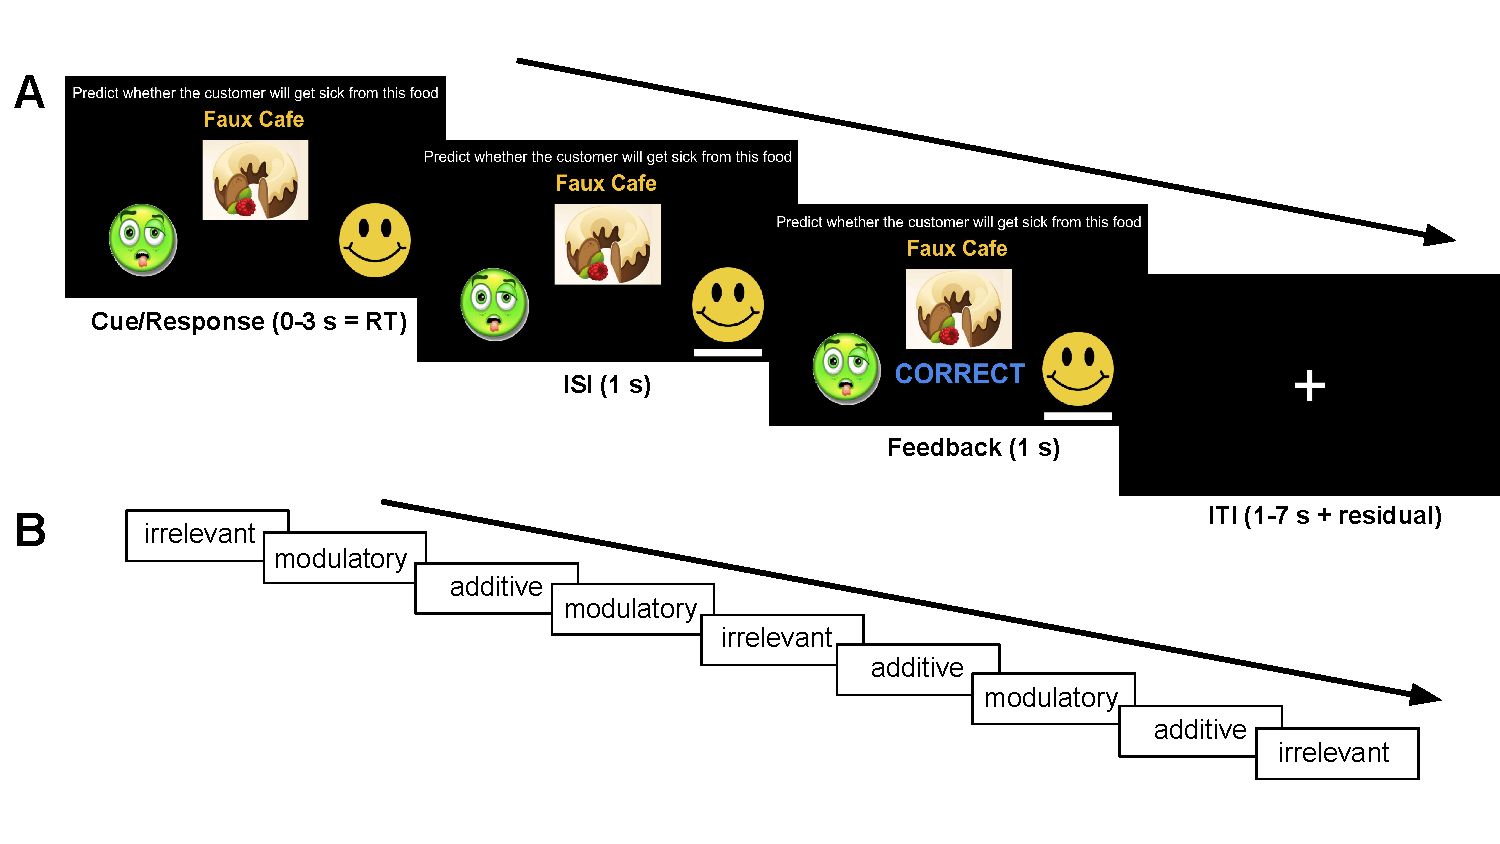
\includegraphics[width=0.5\textwidth]{task-design.pdf}
\end{center}
\vspace{-1em}
\caption{Experimental design. (A) Example timeline of events during a training trial. (B) Example sequence of blocks with the corresponding condition for each block. } 
\label{task-design}
\end{figure}

\subsubsection{Experimental design.} 

We adapted the task used in \citeA{Gershman2017} with a mixed within-subjects design consisting of 9 blocks. Each block consisted of 20 training trials followed by 4 test trials. On each training trial, participants were asked to predict whether a particular food (the cue) in a particular restaurant (the context) would cause sickness (the outcome) and were subsequently informed whether their prediction was correct (Figure~\ref{task-design}A). On each test trial, participants were asked to make a prediction about an old or a novel cue in an old or a novel context, without receiving any feedback, with each of the 2x2 combinations appearing exactly once. In each block, the cue-outcome contingencies depended on the context in accordance with one of the three causal interpretations (irrelevant, modulatory, additive) which we refer to as the condition for that block. The nine blocks were divided in three consecutive groups such that each condition appeared in exactly one block in each group (Figure~\ref{task-design}B). Thus each participant learned under each condition three times. Each block contained a different set of foods and restaurants that were randomized across blocks.
\\

\subsubsection{Simulations.} 

We implemented the model presented in \citeA{Gershman2017}. The model had two free parameters: the variance $\sigma^2_w$ of the Gaussian prior from which the weights are assumed to be drawn; and the inverse temperature $\beta$ used in the logistic transformation from predictive posterior expectation to choice probability. Intuitively, the former corresponds to the level of uncertainty in the initial estimate of the weights, while the latter reflects the exploration-exploitation tradeoff of the model choices. We fit these parameters using maximum likelihood parameter estimation based on behavioral data obtained from 10 different subjects who performed the same task outside the scanner during a pilot version of the study (data not shown). The fitted values were $\sigma^2_w = 0.1249$ and $\beta = 2.0064$. All other parameters had the same values as described in \citeA{Gershman2017}. Each block was simulated independently using the same set of parameters.


\section{Results}

\begin{figure}[ht]
\begin{center}
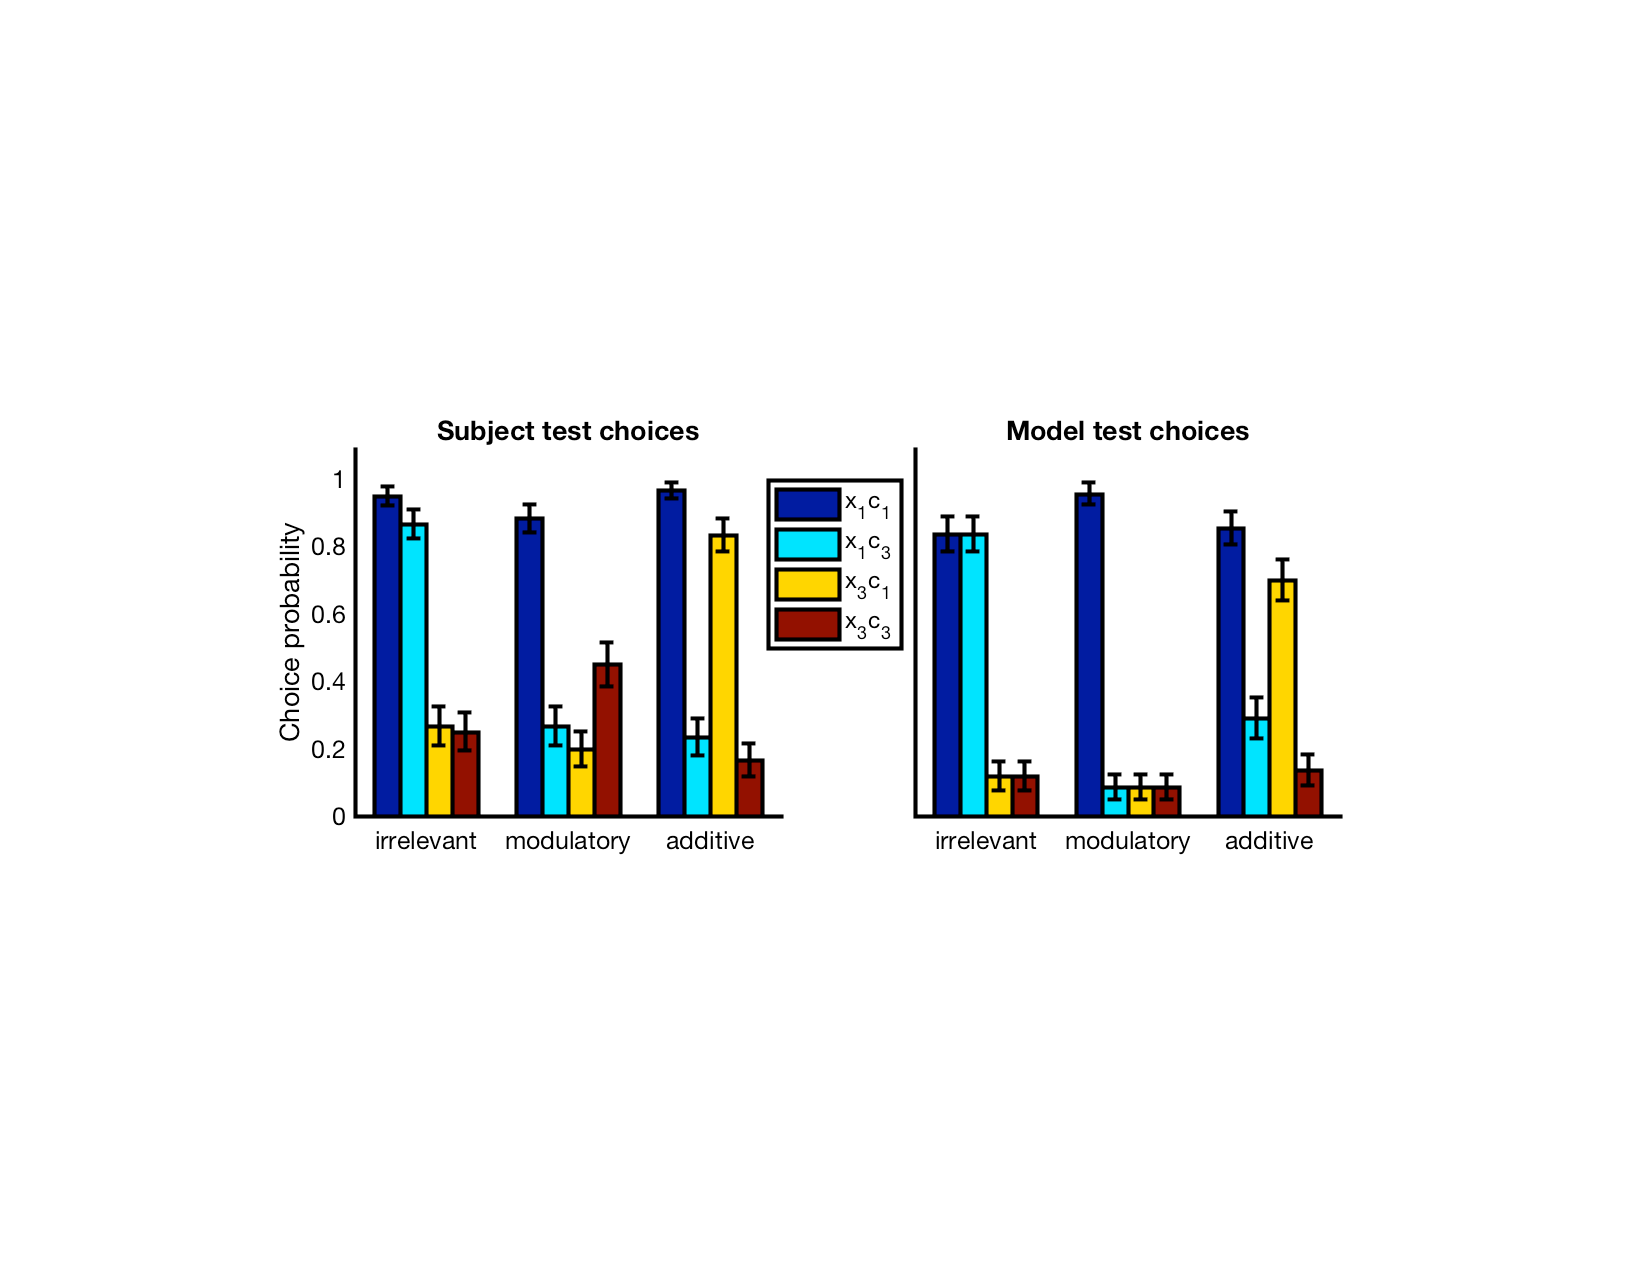
\includegraphics[scale=0.45,  trim = 120 220 120 200]{behavioral.pdf}
\end{center}
\caption{Subject (left) and model (right) performance on the test trials.} 
\label{behavioral}
\end{figure}

\subsubsection{Behavioral performance.}

Test trial choices averaged across blocks are shown in Figure~\ref{behavioral}. Overall, participants learned the task quickly and exhibited the same within-subjects behavioral pattern as was previously reported using a between-subjects design \cite{Gershman2017}. The model successfully accounted for participants' choices on both the training and the test trials ($r = 0.7283, p < 0.00001$) using the parameters obtained from pilot data from a different set of participants.

\begin{figure}[ht]
\begin{center}
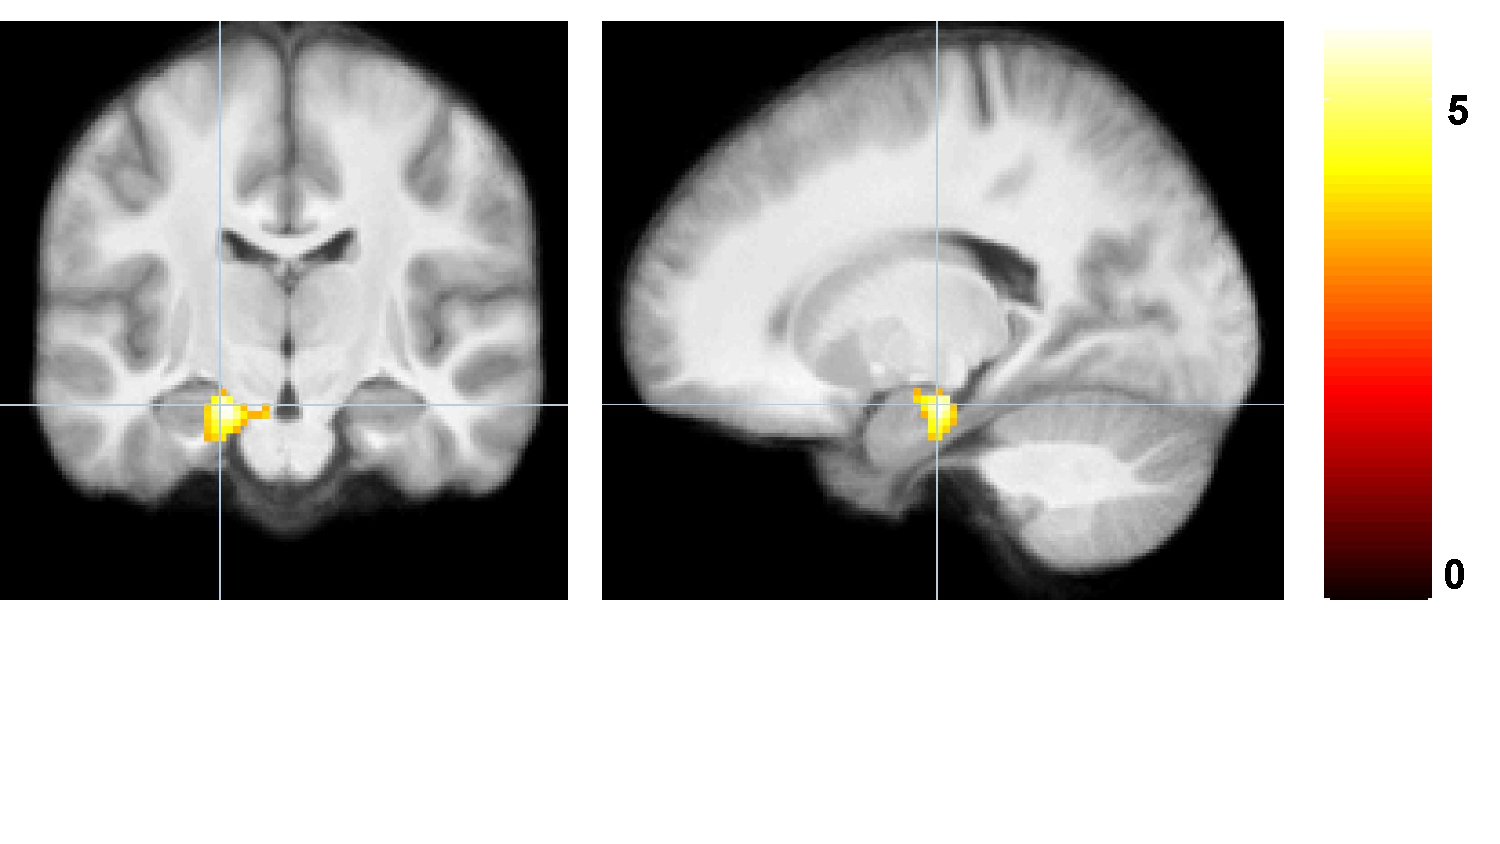
\includegraphics[scale=0.33,  trim = 0 150 0 0]{additive-irrelevant.pdf}
\end{center}
\caption{Transient activity related to the additive condition minus the irrelevant condition in left anterior hippocampus (MNI: -18 -16 -18), $t > 3.5518, p < 0.001$, cluster FWE corr. Right: T-value scale.} 
\label{additive-irrelevant}
\end{figure}

\subsubsection{Imaging data.} 

We had an a priori hypothesis that the hippocampus would be involved in modulating the cue-outcome association when it is influenced by the context. We therefore contrasted BOLD activation between blocks in the different conditions at the time of outcome presentation during the training phase. The BOLD signal did not differ significantly between the modulatory and the irrelevant conditions, nor between the modulatory and the additive conditions. The contrast between the additive and the irrelevant conditions showed increased activation in left anterior hippocampus (Figure~\ref{additive-irrelevant}; MNI coordinates of peak voxel: [-18 -16 -18]; t-value: 5.748; extent with $t > 3.5518$: 141; $p < 0.001$; cluster FWE corrected). Each contrast also included a constant regressor at the time of trial onset to account for the visual activation.

\begin{figure}[ht]
\begin{center}
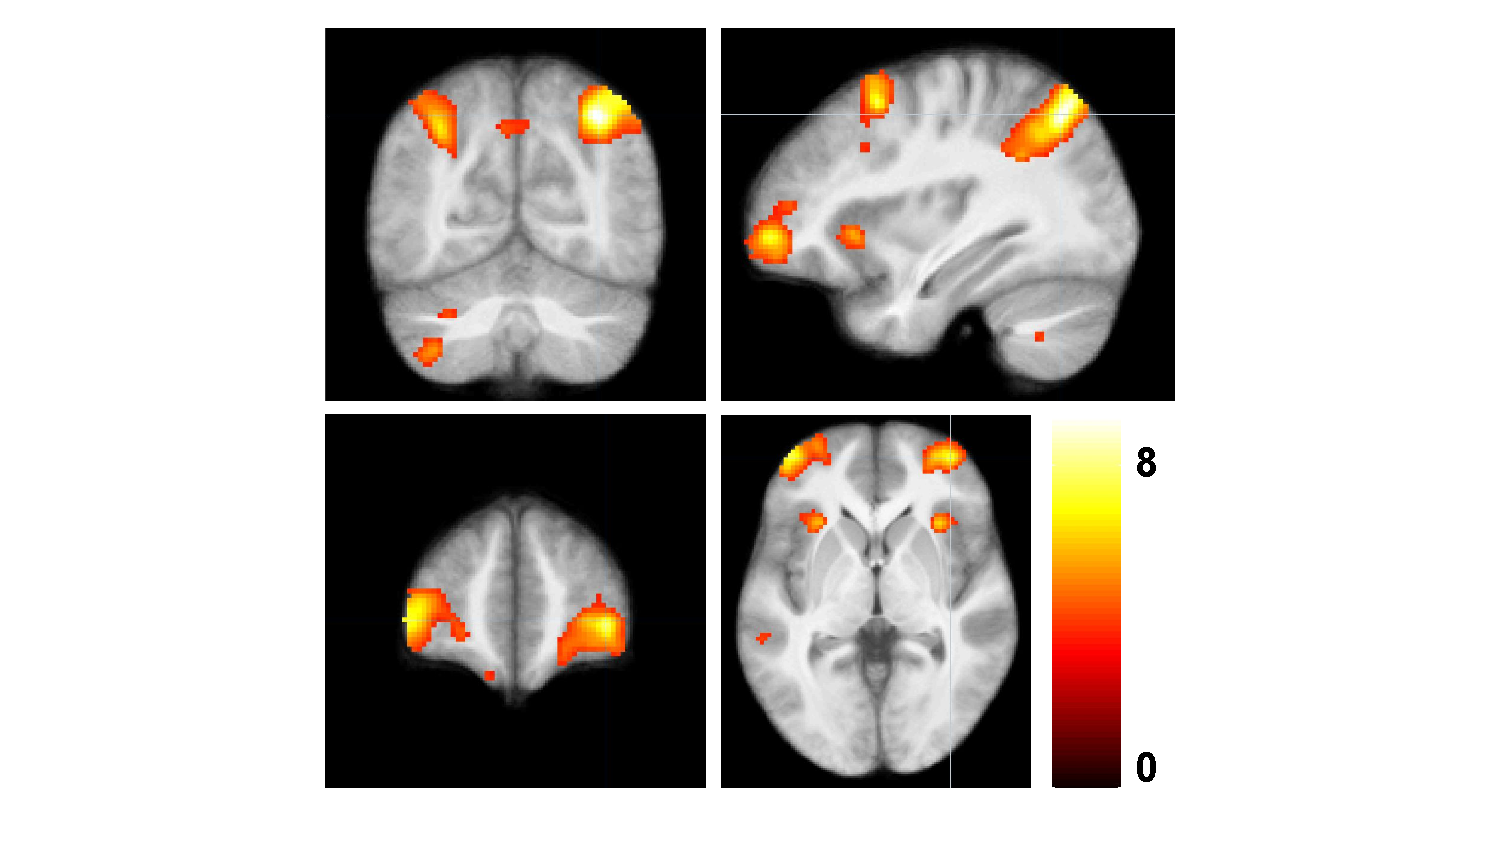
\includegraphics[scale=0.5,  trim = 130 50 0 0]{kl-divergence.pdf}
\end{center}
\caption{Transient activity tracking the Kullback--Leibler divergence of the posterior over causal structures. Top row: right angular gyrus (MNI: 34 -64 48). Bottom row: right rlPFC (MNI: 48 20 34). $t > 3.5518, p < 0.001$, cluster FWE corr. Bottom right: T-value scale.} 
\label{kl-divergence-img}
\end{figure}

In order to measure the neural correlates of structure learning, we computed a contrast with a parametric modulator corresponding to the Kullback--Leibler divergence of the posterior over causal structures which is updated by the model at the time of outcome presentation on each training trial. The results are shown in Table~\ref{kl-divergence-table} and Figure~\ref{kl-divergence-img}. We found significant bilateral activation in parietal cortex (the angular gyri), rostrolateral prefrontal cortex (rlPFC), and anterior insula.

\begin{table}[!ht]
\begin{center} 
\caption{Brain activation tracking the Kullback--Leibler divergence of the posterior over causal structures during training. Only cerebral regions with T-value $ > 5$ are shown. All P-values are $< 0.001$ with cluster FWE correction. Regions were automatically labeled using the AAL2 atlas.} 
\label{kl-divergence-table} 
\vskip 0.12in
\begin{tabular}{llll} 
\hline
Brain region    &  Extent & T-value  & MNI coord. \\
\hline
Angular gyrus (R) &	484	& 8.638 &	34	-64	48\\
Inferior frontal gyrus,\\opercular part (R) &	341 &	8.378& 48	 20	34 \\
Middle frontal gyrus (R) &	130	& 7.440 &	36	56	-2 \\
Middle frontal gyrus (L) &	173	& 7.205 &	-42	56	2 \\
Middle frontal gyrus (R) &	86	& 6.996 &	34	12	54 \\
Inferior parietal gyrus (L) &	254 	& 6.699 &	-30	-54	42 \\
Superior parietal gyrus (L)	 & 254	& 5.566 &	-34	-72	54 \\
Inferior frontal gyrus,\\triangular part (L) &	173	& 6.583 & -44	20	22 \\
Inferior temporal gyrus (R) &	 15	& 6.461 &	60	-24	-20 \\
Insula (L)	& 18	 & 6.272	& -28	22	-2 \\
Anterior orbital gyrus (R)& 	8  &	5.827 &	20	48	-16 \\
\hline
\end{tabular} 
\end{center} 
\end{table}

To find out if other regions contain information related to structure learning, we trained a multinomial classifier based on the generalized linear model (GLM) to predict the condition of a given block based on neural activity from a given region at the time of trial onset. We trained the model on the first 8 blocks and evaluated performance on the last block across all subjects. While performance was at chance level for all regions, the hippocampus showed a significant bias towards predicting the modulatory condition ($p < 0.0001$, one-way repeated-measures ANOVA and post-hoc t-tests) while no bias was observed for other regions (OFC, striatum, and vmPFC, all $p$'s $> 0.01$). To further investigate this trend, we computed a subject-averaged representation dissimilarity matrix (RDM) using correlation distance of activation patterns from different regions at trial onset. This revealed that hippocampal representations of the modulatory condition are more dissimilar from those in the other two conditions ($p < 10^{-6}$, one-way repeated-measures ANOVA and post-hoc t-tests), suggesting that the hippocampus can preferentially distinguish the modulatory causal structure. The same analysis showed that striatum encoded more distinct representations when the context was irrelevant ($p < 10^{-8}$).

\section{Conclusion}

These data suggest that different regions encode information about causal structures reflecting the role that context plays during learning. These results are consistent with previous findings that implicate the hippocampus and the angular gyri in modulating context-dependent associations, with the striatum thought to support a separate stimulus-response learning system.

\nocite{ChalnickBillman1988a}
\nocite{Feigenbaum1963a}
\nocite{Hill1983a}
\nocite{OhlssonLangley1985a}
% \nocite{Lewis1978a}
\nocite{Matlock2001}
\nocite{NewellSimon1972a}
\nocite{ShragerLangley1990a}


\bibliographystyle{apacite}

\setlength{\bibleftmargin}{.125in}
\setlength{\bibindent}{-\bibleftmargin}

\bibliography{ccn_style.bib}


\end{document}
